%| Weekly report template for CSUS Senior Design
%|
%| language: LaTeX
%| Author: Ben Smith
%| 
%| This source has been tagged with the "CHANGE" tag in areas
%| that require updating when making a new docuent
%|
%| This source will generate a PDF file complete with thumbnails navigation menu and metadata.
%| Much of the tex awesomeness comes from http://www.michaelshell.org/ praise be to him for creating the guide
\newcommand{\KEYWORDS}{Logic Gates, Verilog, FPGA, Signaltap, Synthesis}

%| This is a header file for Latex documents  
%| It contains a number of common packages, settings, and custom macros that I frequently use.
\documentclass[9pt,journal]{IEEEtran}

\usepackage[cmex10]{amsmath}        %| American Mathematical Society package for fancy maths  b
\interdisplaylinepenalty=2500              %| Restores IEEE line spacing after amsmath

%| IEEE Citation package
\usepackage{cite}
\usepackage[section]{placeins}
\usepackage{array}
\usepackage{dblfloatfix}
\usepackage{color}
\usepackage{graphicx}
\usepackage{float}
\usepackage{url}                         %| Improved URL handling
\usepackage{etoolbox}
\usepackage[font=footnotesize]{subcaption}
\usepackage{listings}
\usepackage{fixltx2e}               %| Better tables than for LaTeX 2e
\usepackage{minted}

%| Highlighting for source code listings
\definecolor{mygreen}{rgb}{0,0.6,0}
\definecolor{ltgray}{rgb}{0.93,0.93,0.93}
\definecolor{dkgray}{rgb}{0.5,0.5,0.5}
\definecolor{mymauve}{rgb}{0.58,0,0.82}
\lstset{
  backgroundcolor=\color{ltgray},  % choose the background color; you must add \usepackage{color} or \usepackage{xcolor}
  basicstyle=\scriptsize\ttfamily, % the size of the fonts that are used for the code
  breakatwhitespace=true,         % sets if automatic breaks should only happen at whitespace
  breaklines=true,                 % sets automatic line breaking
  captionpos=b,                    % sets the caption-position to bottom
  commentstyle=\color{mygreen},    % comment style
  deletekeywords={...},            % if you want to delete keywords from the given language
  escapeinside={\%*}{*)},          % if you want to add LaTeX within your code
  extendedchars=true,              % lets you use non-ASCII characters; for 8-bits encodings only, does not work with UTF-8
  frame=single,                    % adds a frame around the code
  keepspaces=true,                 % keeps spaces in text, useful for keeping indentation of code (possibly needs columns=flexible)
  keywordstyle=\color{blue},       % keyword style
  language=SystemVerilog,          % the language of the code(I modified the .sty for systemverilog, found the code on google)
  morekeywords={*,...},            % if you want to add more keywords to the set
  numbers=left,                    % where to put the line-numbers; possible values are (none, left, right)
  numbersep=4pt,                   % how far the line-numbers are from the code
  numberstyle=\tiny\color{dkgray}, % the style that is used for the line-numbers
  rulecolor=\color{black},         % if not set, the frame-color may be changed on line-breaks within not-black text (e.g. comments (green here))
  showspaces=false,                % show spaces everywhere adding particular underscores; it overrides 'showstringspaces'
  showstringspaces=false,          % underline spaces within strings only
  showtabs=false,                  % show tabs within strings adding particular underscores
  stepnumber=2,                    % the step between two line-numbers. If it's 1, each line will be numbered
  stringstyle=\color{mymauve},     % string literal style
  tabsize=2,                       % sets default tabsize to 2 spaces
  title=\lstname                   % show the filename of files included with \lstinputlisting; also try caption instead of title
}

\lstset{keywordstyle=\color{purple}}
\lstset{keywordstyle={[2]\color{purple}} }
\lstset{keywordstyle={[3]\color{magenta}} }
\lstset{keywordstyle={[4]\color{teal} }}
\lstset{keywordstyle={[5]\color{violet!40}} }

% Alter some LaTeX defaults for better treatment of figures:
  % See p.105 of ''TeX Unbound'' for suggested values.
  % See pp. 199-200 of Lamport's ''LaTeX'' book for details.
  %   General parameters, for ALL pages:
  \renewcommand{\topfraction}{0.9}  % max fraction of floats at top
  \renewcommand{\bottomfraction}{0.8} % max fraction of floats at bottom
  %   Parameters for TEXT pages (not float pages):
  \setcounter{topnumber}{2}
  \setcounter{bottomnumber}{2}
  \setcounter{totalnumber}{4}     % 2 may work better
  \setcounter{dbltopnumber}{2}    % for 2-column pages
  \renewcommand{\dbltopfraction}{0.9} % fit big float above 2-col. text
  \renewcommand{\textfraction}{0.07}  % allow minimal text w. figs
  %   Parameters for FLOAT pages (not text pages):
  \renewcommand{\floatpagefraction}{0.7}  % require fuller float pages
  % N.B.: floatpagefraction MUST be less than topfraction !!
  \renewcommand{\dblfloatpagefraction}{0.7} % require fuller float pages

%| Enables PDF metadata, thumbnails, and navigation
\newcommand\MYhyperrefoptions{
  bookmarks=true,
  bookmarksnumbered=true,
  pdfpagemode={UseOutlines},
  plainpages=false,
  pdfpagelabels=true,
  colorlinks=true,
  linkcolor={black},
  citecolor={black},
  urlcolor={blue},
  pdftitle={CPE/EEE 64 Lab},
  pdfsubject={Engineering},                        
  pdfauthor={Ben Smith},
  pdfkeywords={Logic Design, FPGA, Verilog}}                       

%| Calls hyperref package with the options specified above
\usepackage[\MYhyperrefoptions,pdftex]{hyperref}

%| Font settings
\renewcommand{\sfdefault}{phv}
\renewcommand{\rmdefault}{ptm}
\renewcommand{\ttdefault}{pcr}

%| Restores IEEE table formatting after usage of subcaption package
\captionsetup[table]{format=plain,labelformat=simple,justification=centering, labelsep=newline, singlelinecheck=false, textfont={sc}}

%| Required Lab Demo custom function
%| \demo{Name}{Physical deliverable}{Documentation deliverable}{Process}
%| =================================================================================================
%| for boxed text and stuch
\usepackage{fancybox}
\newenvironment{fminipage}%
{\begin{Sbox}\begin{minipage}}%
{\end{minipage}\end{Sbox}\Ovalbox{\TheSbox}}

%| Actual bawx
\newcommand{\demo}[4] {
\vspace{15px}
\begin{centering}
  \begin{fminipage}{.47\textwidth}
    \vspace{3px}
    \centering{\bfseries \large Laboratory Demo: #1}\\*
    \vspace{10px}
    \begin{tabular}{p{1.4cm}  p{6.3cm}}
      %|==Requirements for lab demo==
      \raggedright Specification:                  &#2\\
      \\
      \raggedright  Deliverable:                   &#3\\
      \\
      \raggedright Process :                       &#4\\
    \end{tabular}
  \end{fminipage}
\end{centering}
}

%| Single figure
%| \small{Location}{Caption}{Label}
%| =================================================================================================
\newcommand{\smallfig}[3] {
  \begin{figure}[H]
    \includegraphics[width=.48\textwidth]{#1}
    \caption{#2}
    \label{#3}
  \end{figure}
}

%| Single figure
%| \simpletable{c||c}{Caption}{Label}{content}
%| =================================================================================================
\newcommand{\simpletable}[4] {
  \begin{table}[!t]
    \caption{#2}
    \label{#3}
    \centering
    \begin{tabular}{#1}
      \hline
      #4
    \end{tabular}
  \end{table}
}

\begin{document}
\title{Lab Two: Introduction to logic on the FPGA}
\author{Ben Smith}
\maketitle

  \begin{abstract}
    This document is an introduction to the DE0-Nano development board, Altera's Cyclone FPGAs and the Quartus IDE. The block editor feature of Quartus is used to synthesize logic gate primitives and more complex logic functions from these primitives.
  \end{abstract}

  %| =================================================================================================
  %| Introduction
  %| =================================================================================================
  \section{Introduction}
    \PARstart{T}{his} lab introduces the DE0-Nano development board and Altera's Quartus development environment. Quartus will be used to program the Altera Cyclone IV FPGA on the DE0-Nano.\footnote{\href{https://www.youtube.com/watch?v=gUsHwi4M4xE}{EEV Blog: What is a FPGA?} Take a look at this page for a great explanation of what FPGAs are all about, even if a kangaroo delivers the speech. So mount that wallaby and get some understanding} We will start by using Quartus' schematic representation of logic modules and move into text based design capture. The schematic entry method his will be very similar to the logic designs that you have created in Multisim and implemented with discrete 7400 series logic ICs. The schematic editor in Quartus can be used to graphically represent Verilog modules as well, like you will do in Lab Two, or logic primitives like will be done in this lab. This lab is intended to introduce the student to the following concepts.
    \begin{itemize}
       \item Logic primitives on a FPGA
       \item Quartus development environment
       \item Synthesis of a block based design
       \item Assigning pins for a design
       \item Programming an Altera FPGA
    \end{itemize}

    \subsection{Included Screencasts}
      A number of screencasts are included with this set of labs. They are available on Youtube and as zipped MP4s on the course website. They are intended to be short and to the point so they cover individual topics.
      \begin{enumerate}
        \item TIME - Installing Quartus
        \item TIME - Opening, Compiling, programming with Quartus
        \item TIME - Block editor in Quartus
        \item TIME - Using the generated pin assignments from the TerasIC system builder
      \end{enumerate}

    \subsection{DE0-Nano Development board}
      The DE0-Nano has a number of devices built into the board to expand the capabilities of the FPGA. Most of these will be beyond the scope of the course but represent real world design challenges and are worth experimenting with after this basic course is completed. Altera offers a number of tutorials for anyone interested in learning more. These labs will use one of the 40-pin GPIO headers to interact with the outside world. 
      \begin{figure}[htpb]
        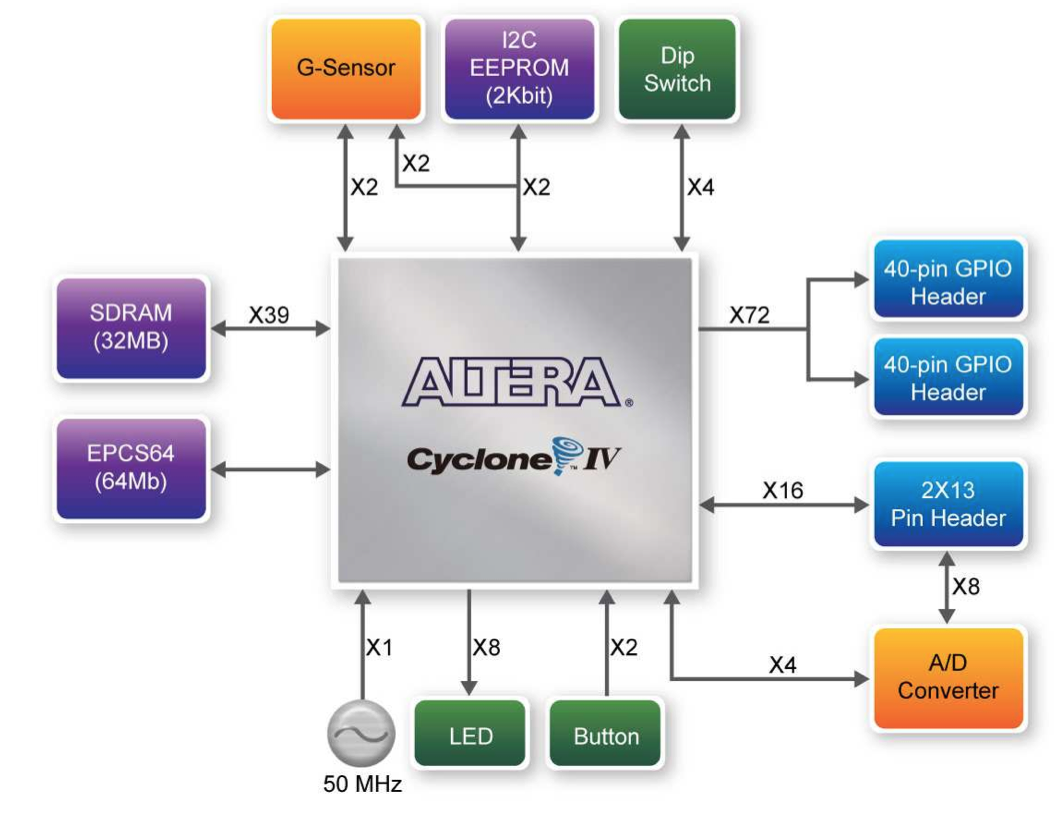
\includegraphics[width=.48\textwidth]{Images/DEONanoBlockDiagram.png}
        \caption{Block Diagram of DE0-Nano \cite{DE0Manual}}
      \end{figure}
      The A/D converter and G-sensor will be great tools to interact with sensors in your later classes. If you choose to go down a path of controls engineering FPGAs will be a great way to implement ``deterministic'' control systems. Interfacing with these components will require the implementation of a SPI or I2C bus protocol. This is done in Verilog just like what we'll do in Lab Two. The De0-Nano system CD comes with some example code that uses these devices. 

  %| =================================================================================================
  %| Procedure
  %| =================================================================================================
  \section{Lab Procedure}
    \PARstart{T}{his} section is a guide for what must be accomplished in the lab. Keep in mind the some of the following material will need to be documented in your lab report. It would behoove you to take a look at the lab report section before starting the procedure. Knowing what you need to record in the experiment will be very important to you. For this section you will need:
    \begin{itemize}
      \item De0-Nano Development board
      \item A breadboard
      \item Four LEDs
      \item Two dip switches
      \item Windows or Linux based computer
      \item Internets
    \end{itemize}

    %| Step Zero: Install Quartus
    %| =================================================================================================
    \subsection{Optional: Install Quartus}
    You can download the most recent version of Quartus and Cyclone device drivers from Altera. Screencast 1
    is a walk through for windows, but Quartus is also available for Linux. This is preinstalled on the computers in the Digital design laboratoy. The same version is available from Altera free of charge if you would like to use your own computer.

    %| Step One: Expand source .zip
    %| =================================================================================================
    \subsection{Expand Source.Zip}
    The Quartus project file and top level schematic are contained within this archive. Expand it wherever is convenient for you, it will be accessed frequently. The Quartus project file included with the source code is generated with the Terasic DE0-Nano System Builder that is included with the Terasic System CD. You can use this if you want to generate a clean project for yourself. The contents of the Zip are explained below, it is from the perspective of the root of the archive.

    \begin{enumerate}
    \item Folder: Quartus Project \\
      The quartus project file is contained in here with the myriad of required support files, generated reports, and logfiles.
    \item Folder: Source Code \\
      The Quartus project references these files. I choose to store them outside of the quartus project file so they are easy to access.
      \begin{enumerate}
        \item 64Lab1.bdf: top level schematic that will be used to capture logic designs
        \item .SV: System Verilog source file
        \item .V: Verilog source file
      \end{enumerate}
    \end{enumerate}
    these files are used to save you some of the tedium of setup. It's worth attempting to create your own project, A tutorial has been included called ScreencastX.
    
    %| Step Two: Open Quartus project
    %| =================================================================================================
    \subsection{Open Quartus project}
    Navigate to where you expanded the Source.zip file. The Quartus project file you want to open is called
    ``./Verilog/Quartus Project/64LabOne.qpf''\footnote{The ./ refers to the root of the source.zip package} When you open the project file open the ``Top Level'' .BDF file
    Inside this file there will be a number of logic gates attached to pins of the FPGA. A screen cast explains the
    intricacies of the Schematic editor. 
    \begin{figure}[htpb]
      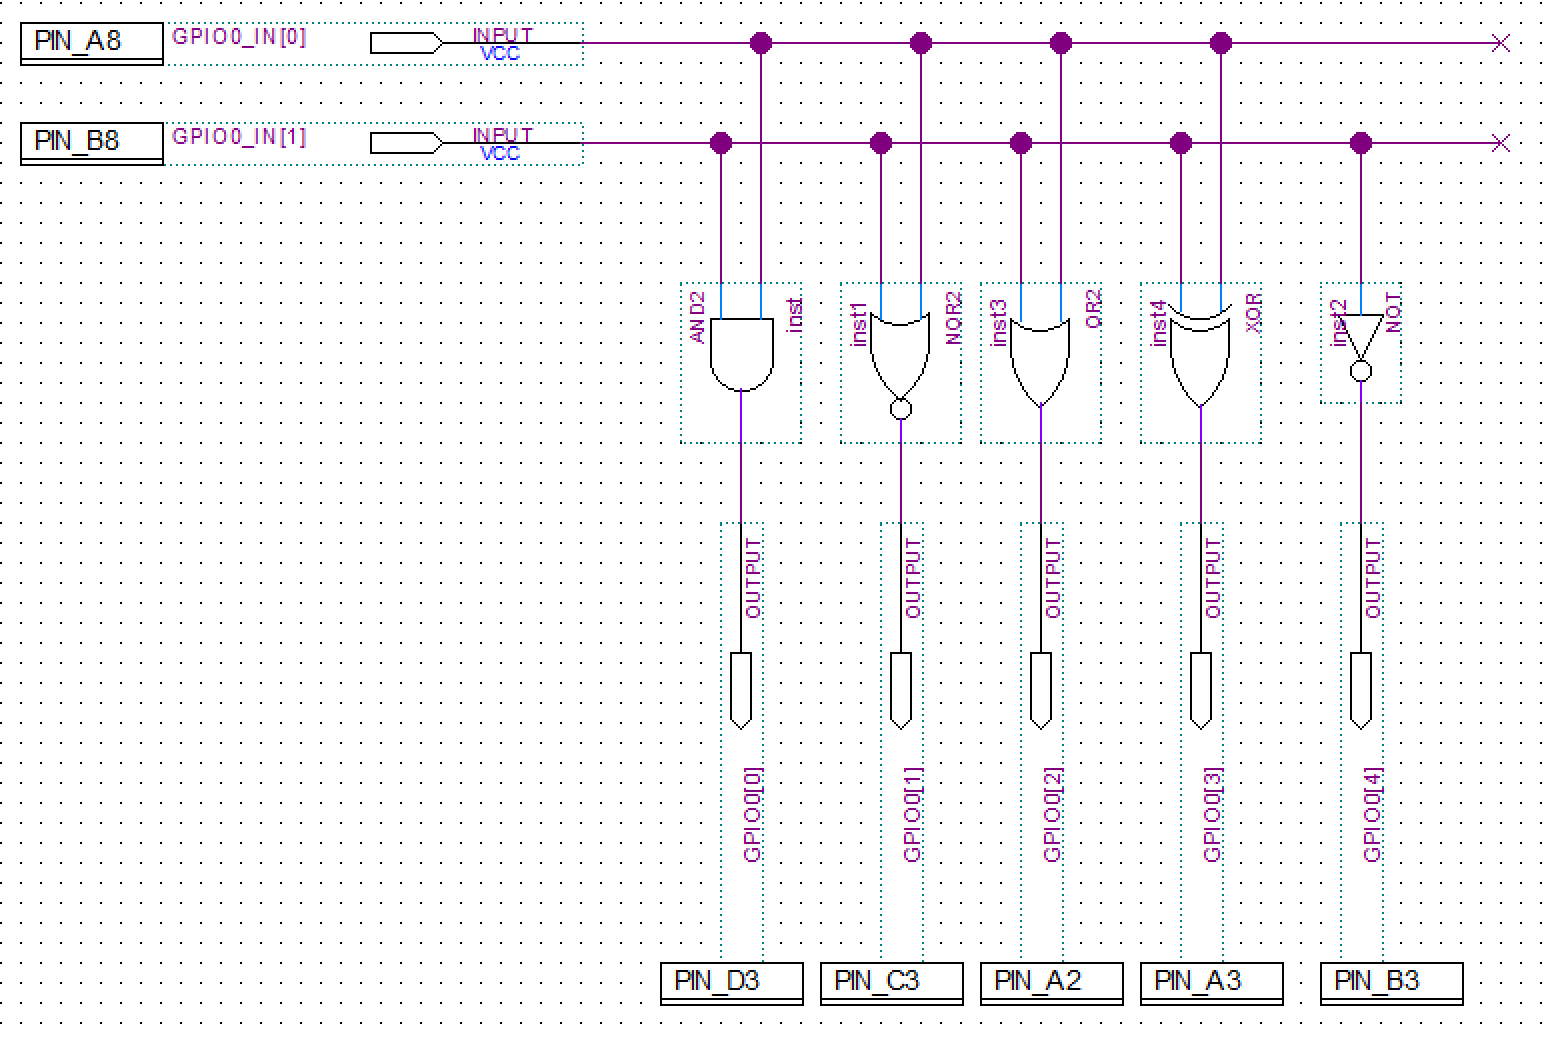
\includegraphics[width=.48\textwidth]{Images/LogicPreview.png}
      \caption{Quartus logic schematic editor example}
    \end{figure}

    %| Step Three: Prepare circuit
    %| =================================================================================================
    \subsection{Prepare circuit to test Verilog gate modules with DE0-Nano}
      A switch and LED are going to be used to test the FPGA while it's operating. This switch will allow you to generate inputs for the FPGA. The LED circuit needs a current limiting resistor as shown in the Figure below.
      \begin{figure}[htpb]
        \label{LEDCircuit}
        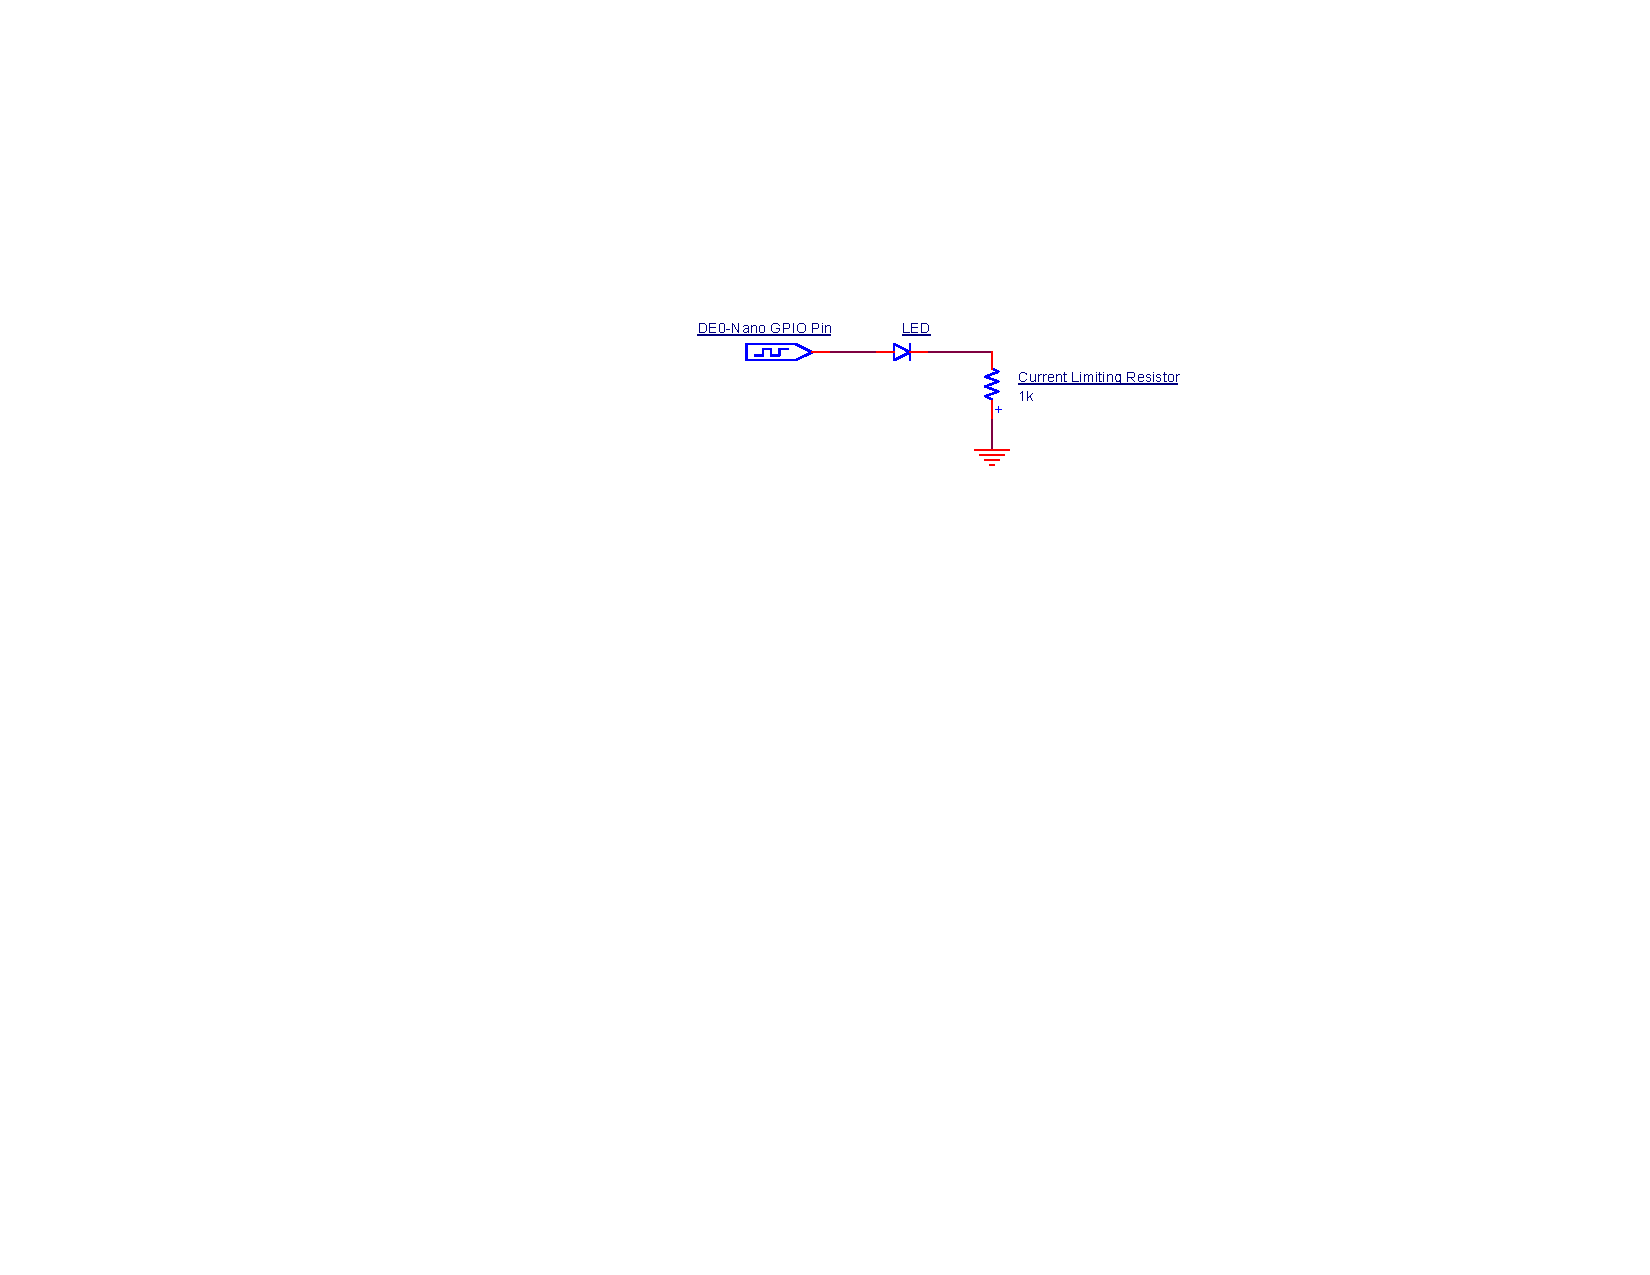
\includegraphics[width=.48\textwidth]{Schematics/LED.pdf}
        \caption{LED with current limiting resistor}
      \end{figure}
      The LED will allow you to see the the output but we'll also need to be able to generate some input for
      the FPGA. We will do this with a dip switch and pulldown resistor. The pulldown resistor is needed
      to literally pull the charge off the wire so the input will read a solid zero. Otherwise the pin would ``float'' between 1 and 0 arbitrarily.

      \begin{figure}[htpb]
        \label{swPulldown}
        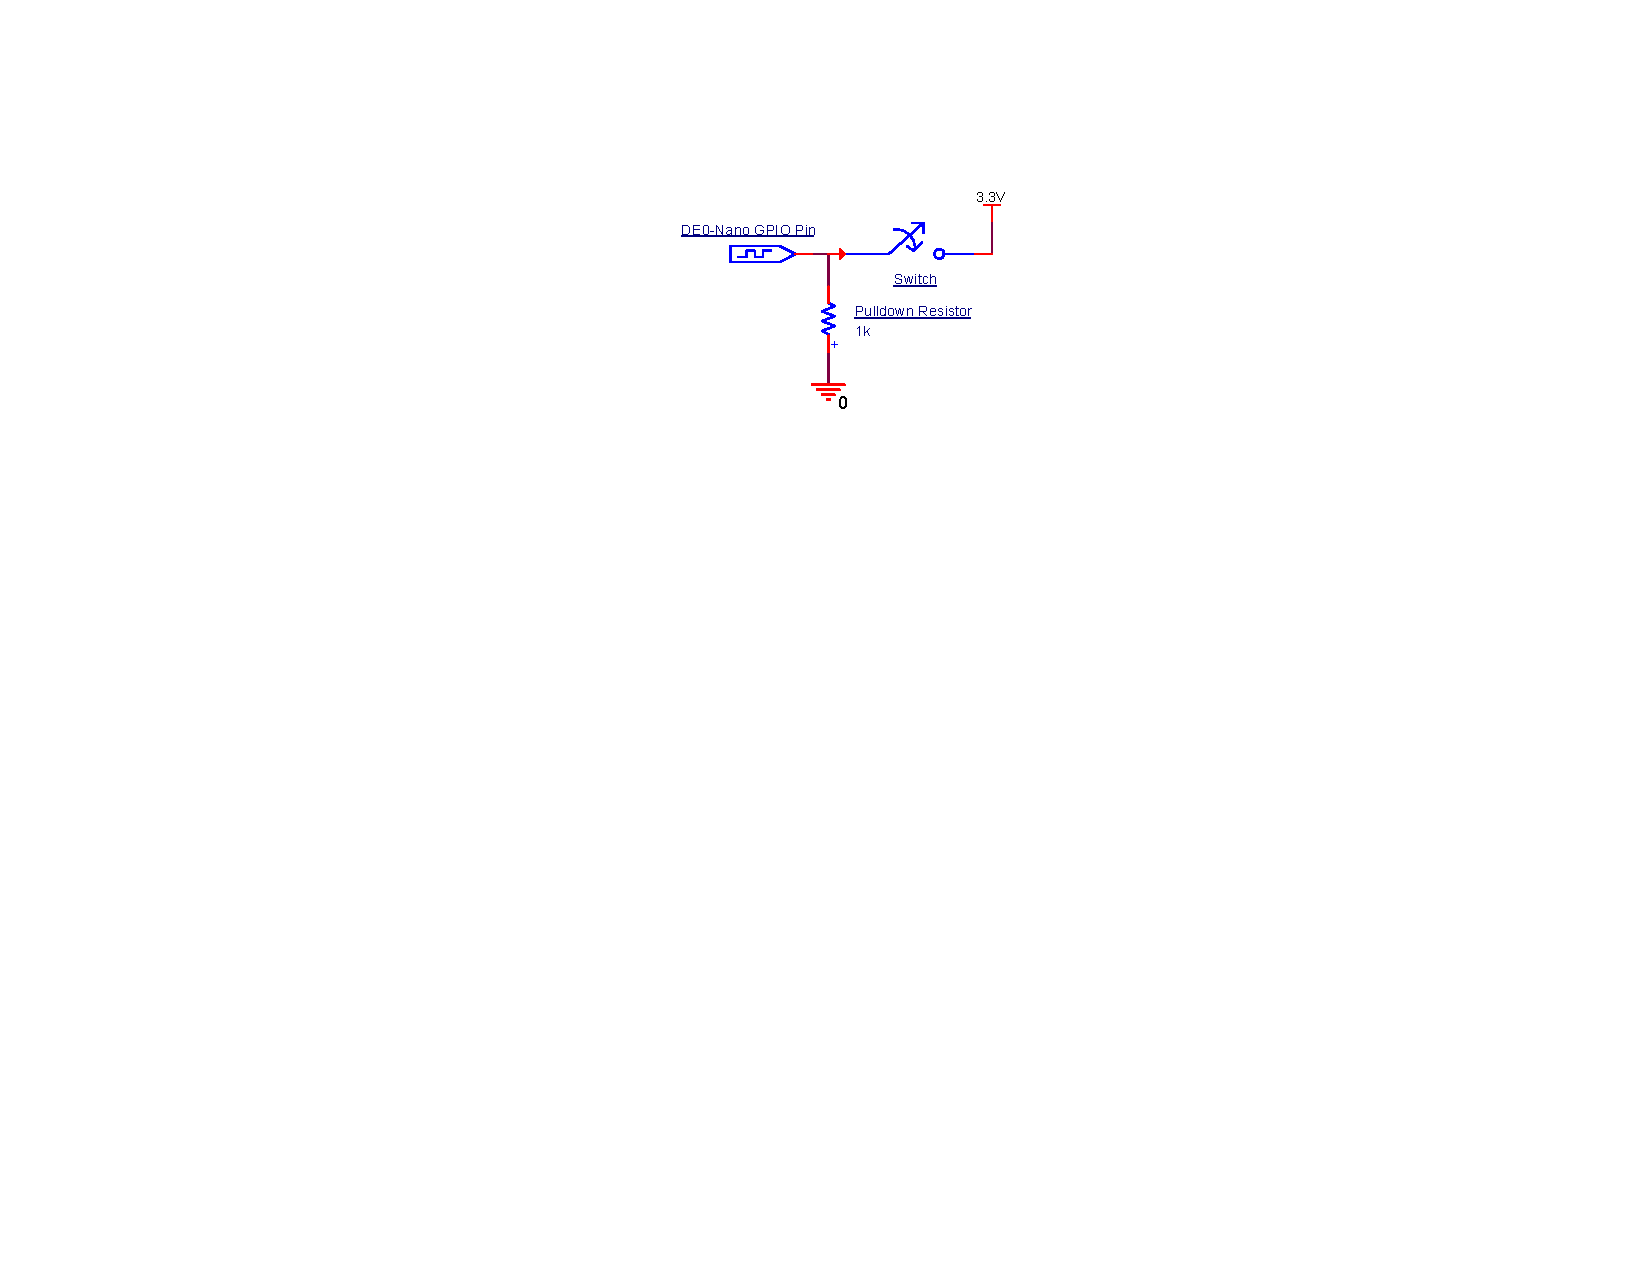
\includegraphics[width=.38\textwidth]{Schematics/SwitchCircuit.pdf}
        \caption{Switch with pulldown resistor}
      \end{figure}

      %| GPIO Headers
      \subsubsection{GPIO headers on the DE0-Nano} 
        Be careful when referencing the pin diagrams in the DE0-Nano user manual. It is easy to read it backwards and that can be a mistake that will cost you hours. It is easiest to match the Nano's orientation with the schematic and count from the nearest edge. Figure \ref{pinmap} shows GPIO 0 next to a schematic of the header. Always check VCC\_SYS, VCC3P3, and GND with a multimeter before attaching a circuit you have built. 
        \begin{figure*}
          \centering
          \begin{subfigure}[b]{.38\textwidth}
            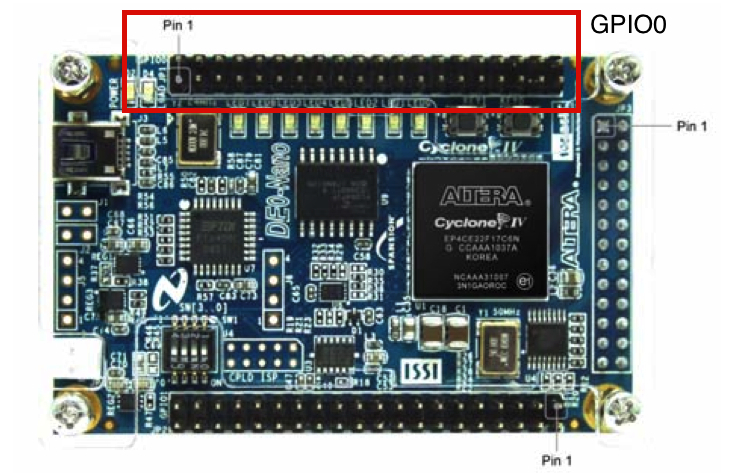
\includegraphics[angle=270, width=.9\textwidth]{Images/LabeledGPIOHeaders.jpg}
            \caption{Orientation of GPIO Header\cite{DE0Manual}}
          \end{subfigure}
          \begin{subfigure}[b]{.45\textwidth}
            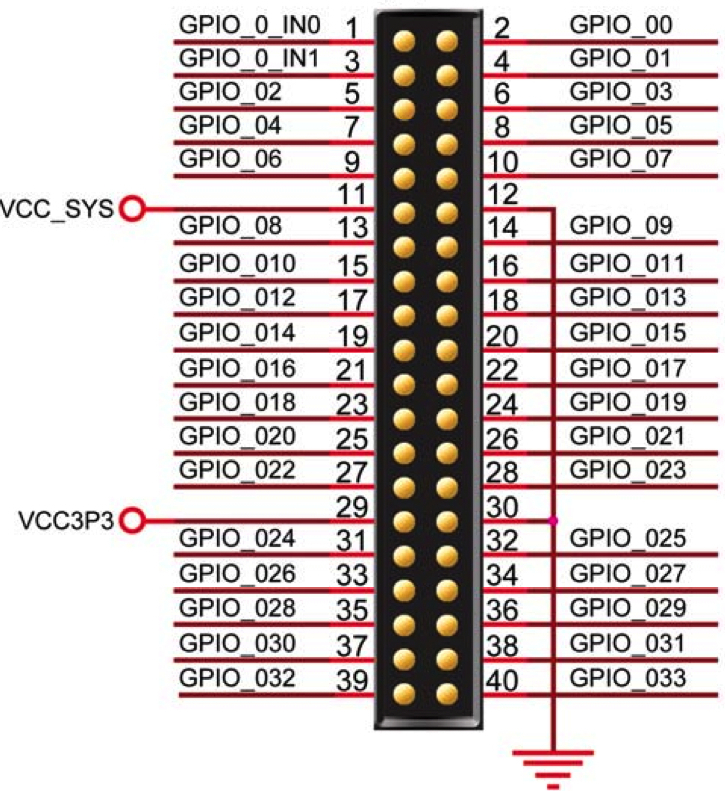
\includegraphics[width=\textwidth]{Images/GPIOHeader.jpg}
            \caption{Schematic of GPIO-0 header\cite{DE0Manual}}
          \end{subfigure}
          \caption{GPIO0 and it's orientation of the development board}
          \label{pinmap}
        \end{figure*}
        This is the header pin schematic from the DE0-Nano user manual. Inside the verilog code these pins follow a little different nomenclature. What is labeled as GPIO\_0\_IN[0] in figure 5 is GPIO0\_IN[0] and GPIO\_00 is GPIO0[0]. Refer to the DE0-Nano user guide for details on the orientation of the headers.

        \begin{figure}[htpb]
          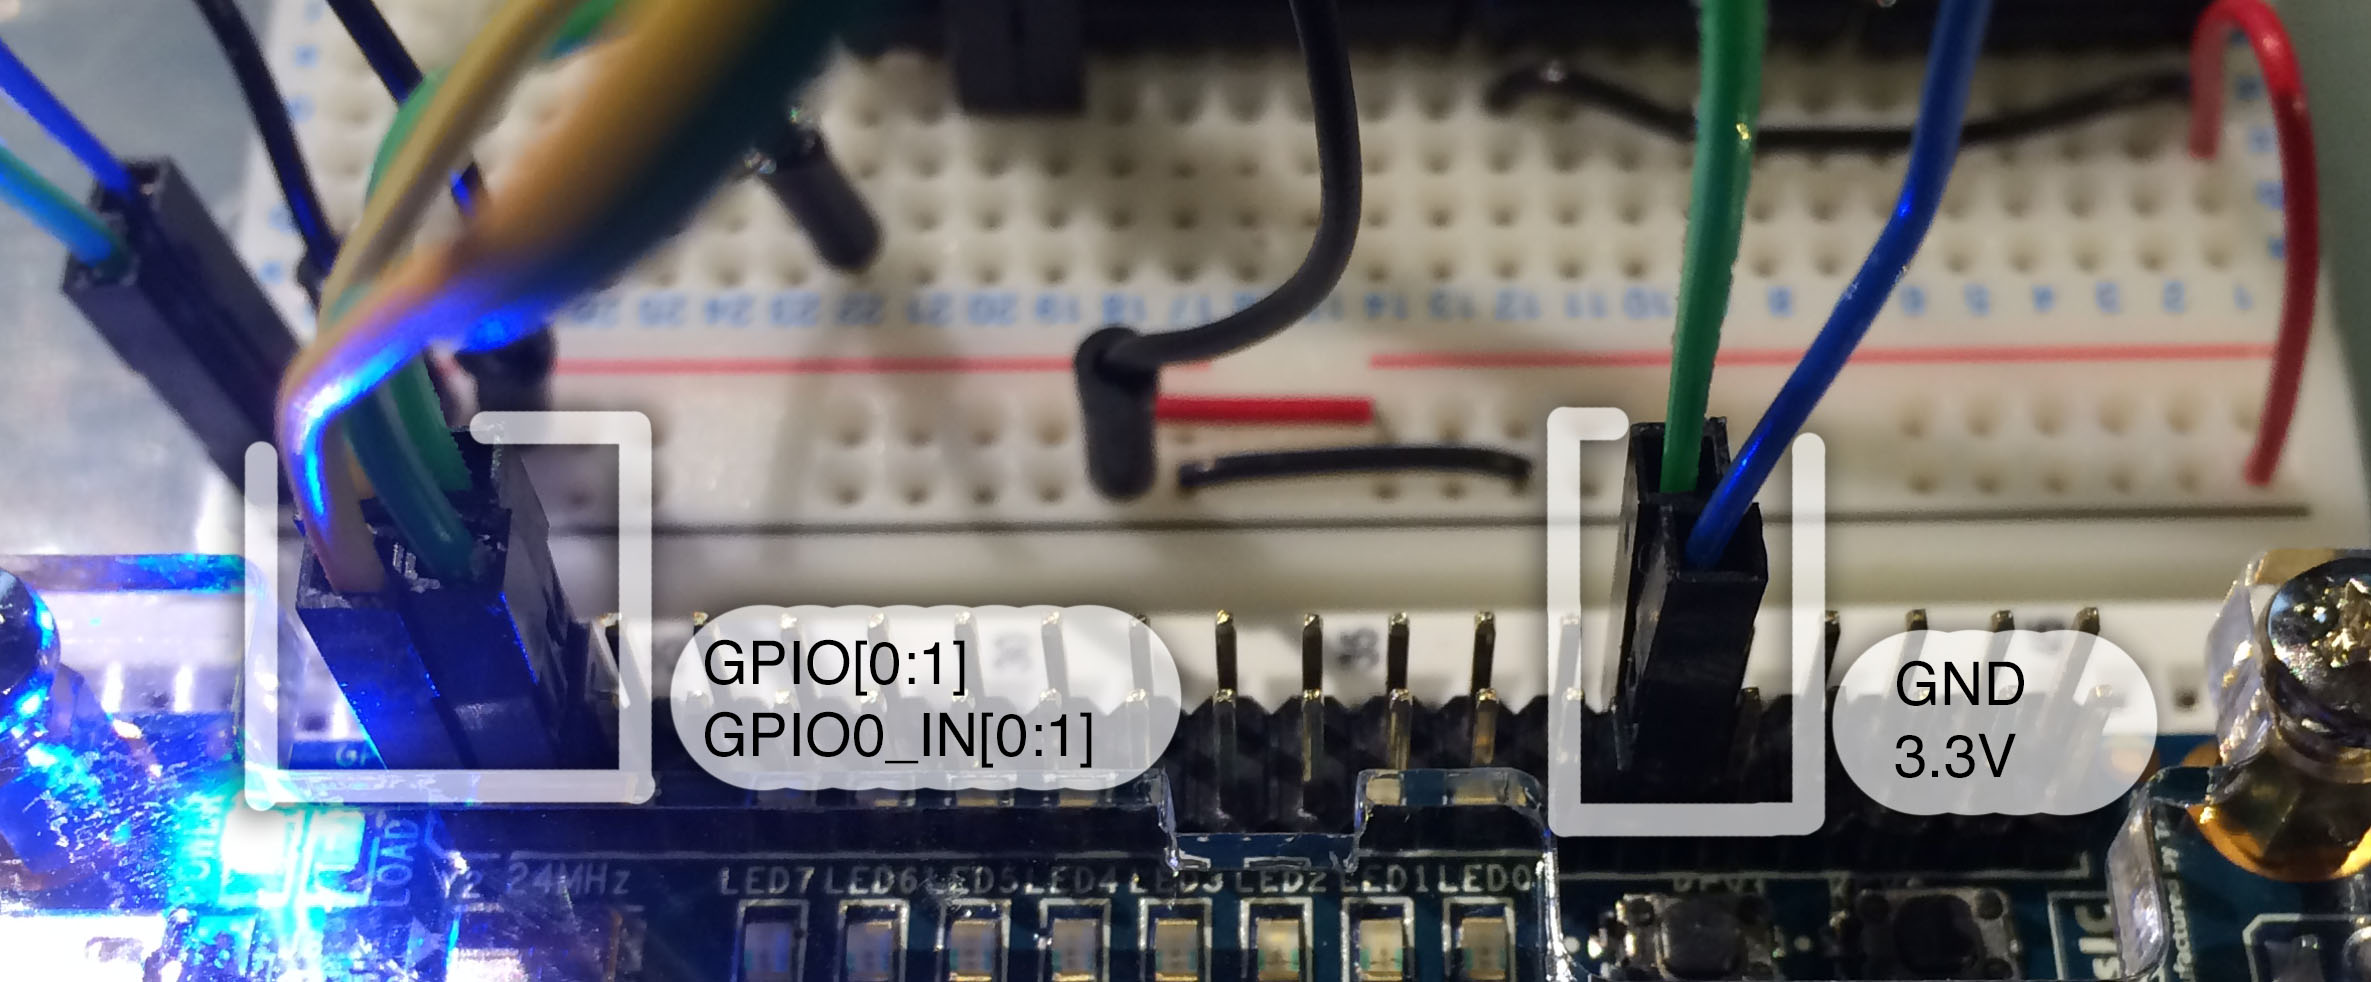
\includegraphics[width=.45\textwidth]{Images/GPIOpicture.jpg}
          \caption{Picture of loaded GPIO-0 header}
        \end{figure}

        \begin{figure}[htpb]
          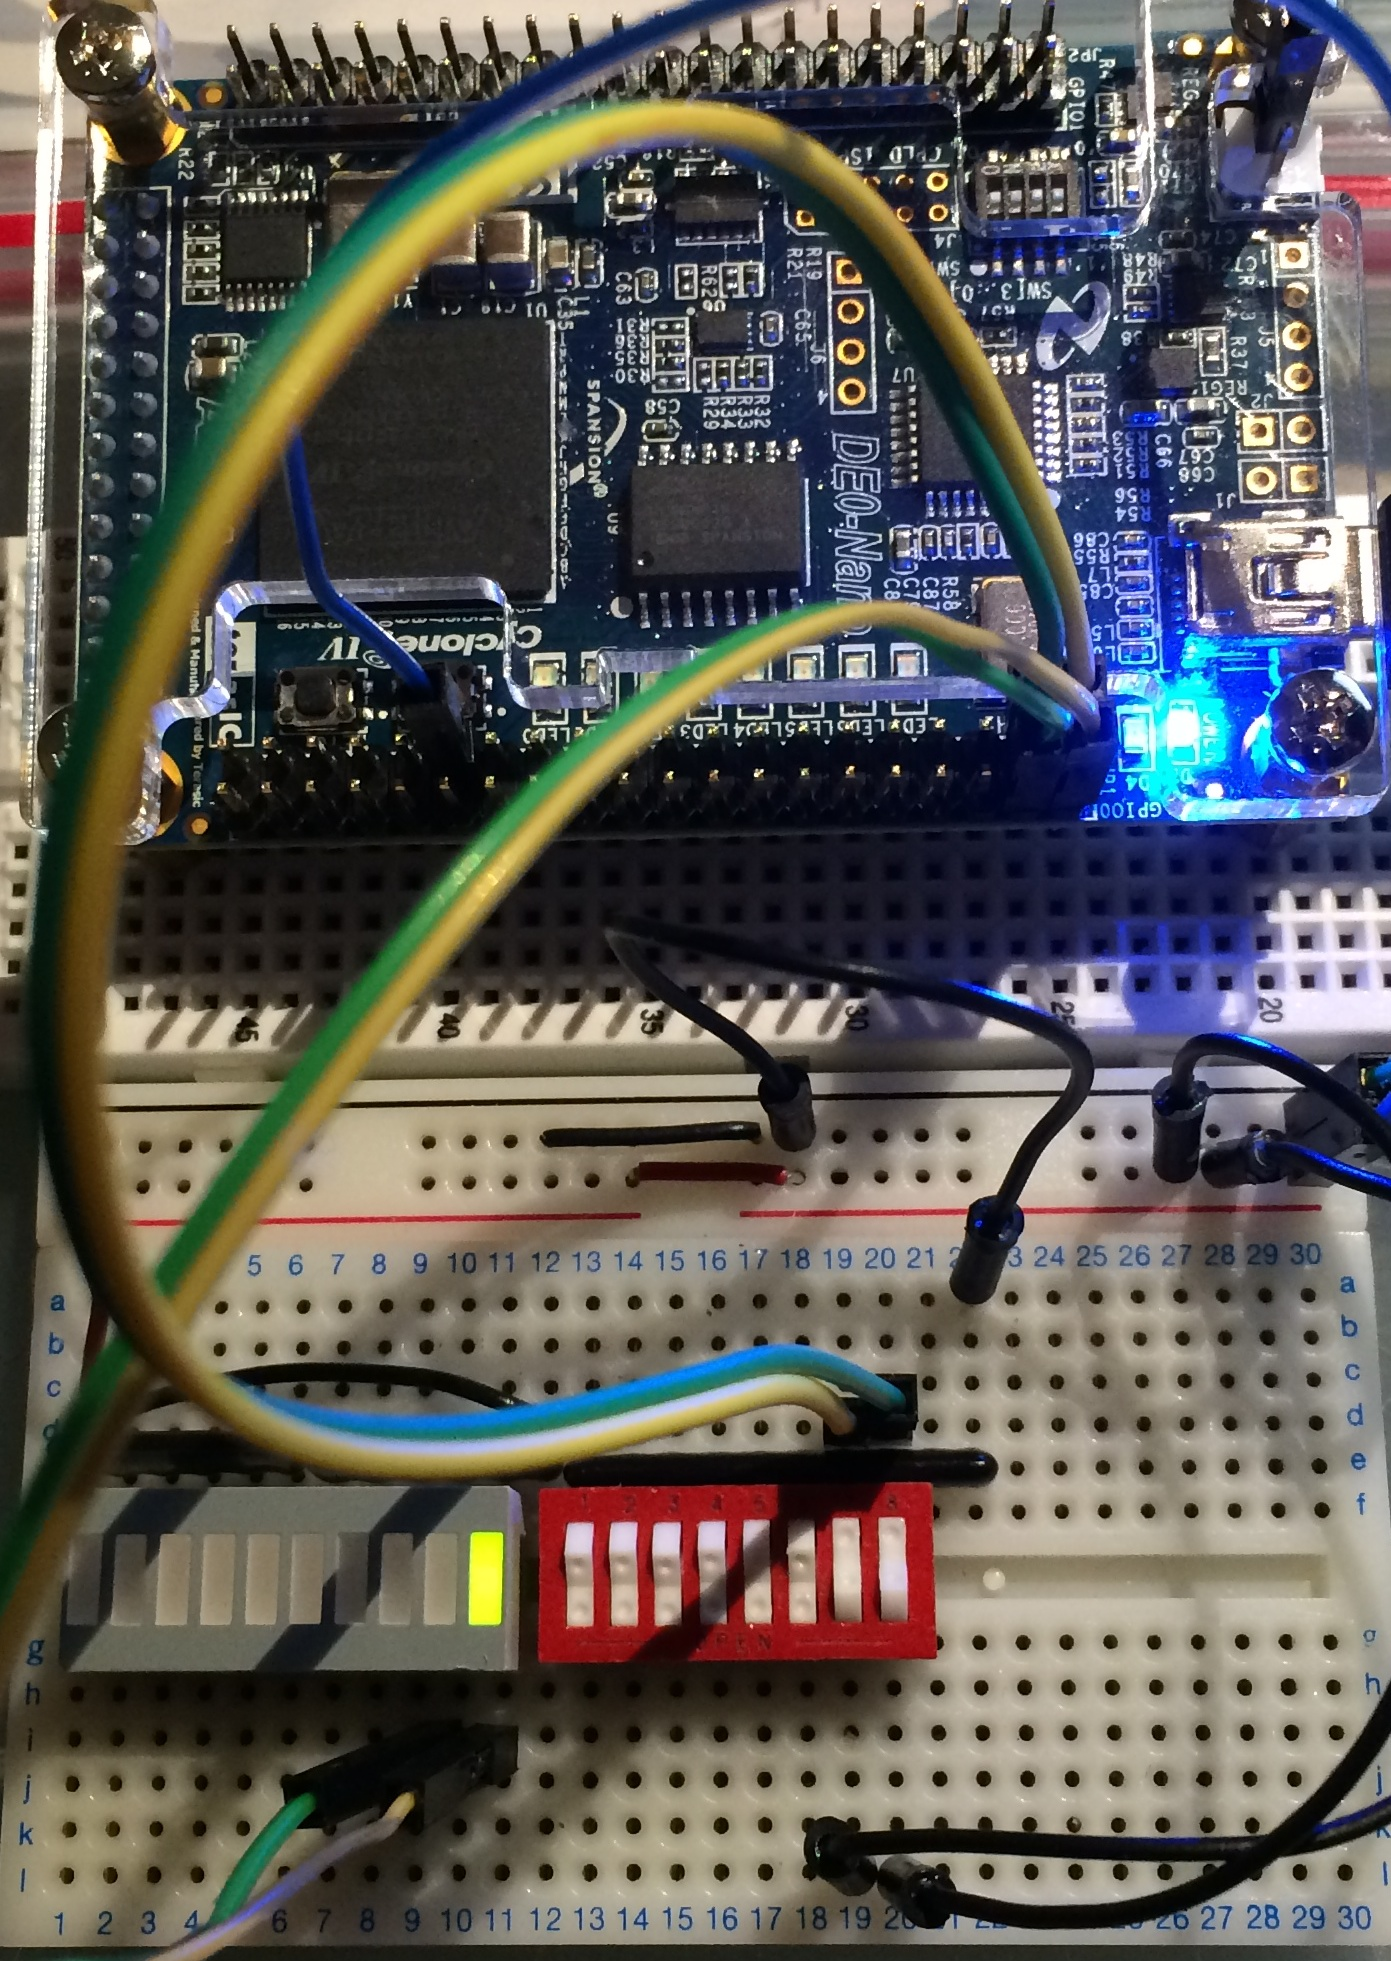
\includegraphics[width=.48\textwidth]{Images/ExampleLayout.jpg}
          \caption{Example switch and LED configuration with SIP resistors}
        \end{figure}

      %| Step Five: Compile
      \subsubsection{Compile example with Quartus}
        Once you've created and tested your switch circuit we'll need to compile the example project. This can be done
        with the Quartus development environment. A walk through is provided in screencastX. 

      %| Step Six: Program Nano
      \subsubsection{Use Quartus to program the Nano} refer to screencastX for a walk through. After synthesis Quartus will generate a .SOF\footnote{the .SOF stands for SRAM object file. This is an Altera standard for of their FPGAs.} file that can be used to program the FPGA using Quartus' programmer.

      %| Step Seven: Record Results
      %| =================================================================================================
      \subsection{Test behavior against expected truth table} 
      Use the known behavior of the logic gates to test your design on the FPGA. It is imperative that you always verify the operation of a design. This design can be verified by creating a Logic Table for each of the gates. If the LED and switch behaves as expected, record the experimental data and move on. If not the design will have to be debugged.

      %| Step Eight: Create XOR from logic primitives
      %| =================================================================================================
      \subsection{Design XOR module} 
        Now that you have had the opportunity to experiment with the logic primitives in the schematic editor the time has come to create your own design. Lets say that we need a four input XOR gate for some reason. We know the truth table of a XOR gate, it must be high when any number of the inputs is high but all of them as shown in Table \ref{XORTT}. Quartus does have an embedded XOR primitive which the use of is disallowed. Create the circuit from the basic 7400 series logic operators(AND, OR, NOT, NAND). Always remember, Google is your best friend. 
        \begin{table}[htpb]
          \renewcommand{\arraystretch}{1.3}
            \caption{Truth table for XOR logic function}
            \label{XORTT}
            \centering
            \begin{tabular}{c|c|c|c|c}
            \hline
              A &B &C &D &Output Q \\
            \hline\hline
              0 &0 &0 &0 &0\\
              0 &0 &0 &1 &1\\
              0 &0 &1 &0 &1\\
              0 &0 &1 &1 &1\\
              0 &1 &0 &0 &1\\
              0 &1 &0 &1 &1\\
              0 &1 &1 &0 &1\\
              0 &1 &1 &1 &1\\
              1 &0 &0 &0 &1\\
              1 &0 &0 &1 &1\\
              1 &0 &1 &0 &1\\
              1 &0 &1 &1 &1\\
              1 &1 &0 &0 &1\\
              1 &1 &0 &1 &1\\
              1 &1 &1 &0 &1\\
              1 &1 &1 &1 &0\\
            \hline
            \end{tabular}
          \end{table}
          Be sure to include a boolean logic expression for this truth table in your report.

      %| Step Eight: Create XOR from logic primitives
      %| =================================================================================================
      \subsection{Design AOI module from logical equation} 
      The ``And or Invert'' function is common in digital design, you will implement it with logic primitives in the schematic editor. There will be a wealth of information available on line about how to implement the function on the Internet but take a stab at it before heading to Google. 

      \begin{displaymath}
        F = \overline{(A \wedge B) \vee (C \wedge D)}
      \end{displaymath}

      Be sure to include a truth table in your lab report.

  %| =================================================================================================
  %| Lab Report Requirements
  %| =================================================================================================
  \section{Lab Report}
    \IEEEPARstart{T}{he} lab report must be typed and submitted in a PDF format. Look to IEEE's guidelines for  guidelines on format. The document should include the following items.
    
    \subsection{Figures to include}
    \begin{itemize}
      \item Schematic of your XOR Gate
      \item Logic tables from theoretical prediction and experimental outcome
      \item Explanation and schematic of your XOR module.
      \item Explanation and Schematic of your AOI module.
    \end{itemize}

    \subsection{Questions to answer}
    \begin{enumerate}
      \item Notice the report that pops up when you compile your project. There are a number of statistics given by Quartus, the logic element usage ratio is your designs use of the total device capacity. What was the logic usage of your FPGA?
      \item The synthesis engine in Quartus is very powerful and will optimize your design for the resources on the   FPGA. Quartus generates the design using three logic gates and two inverters, which gate do you think it changed to inverters?
    \end{enumerate}

  %| =================================================================================================
  %| Conclusions
  %| =================================================================================================
  \section{Conclusion}
    \IEEEPARstart{T}{this} lab introduced Quartus and some of it's basic functionality. Quartus is very similar to many industry standard tools. Xilinx, another manufacturer of programmable logic devices, offers a tool suite very similar to Quartus called ISE. Although we will not discuss ISE, a understanding of Quartus will allow ISE to be learned very quickly. These are tools that you can expect to see in industry as a CPE or EEE student. There is an extreme demand right now for engineers with an understanding of programmable logic.

  %| =================================================================================================
  %| Bibliography
  %| =================================================================================================
  \bibliographystyle{IEEEtran}
\bibliography{IEEEfull}


\end{document}